\chapter{Exporting \trnsys models as FMUs}

\section{Including \type in a \trnsys model}
\label{sec:export:model}

To export a \trnsys model as FMU for Co-Simulation, \type has to be properly included into the model.
\type comes in two variants:
\begin{itemize}
  \item \textbf{\typea}: \emph{Inputs to} the FMU (from the master algorithm) are this type's outputs.
  \item \textbf{\typeb}: This type's inputs are the \emph{outputs from} the FMU (to the master algorithm).
\end{itemize}
The inputs and outputs of the FMU are defined via the \emph{special cards tabs} of \typea and \typeb. In case the information in these tabs is missing (or incomplete), the resulting FMU will not work properly!

Figure~\ref{fig:trnsys_model} shows a screen shot from Simulation Studio with a simple \trnsys model that includes an instance of \typea and \typeb.

\begin{figure}[h]
\centering{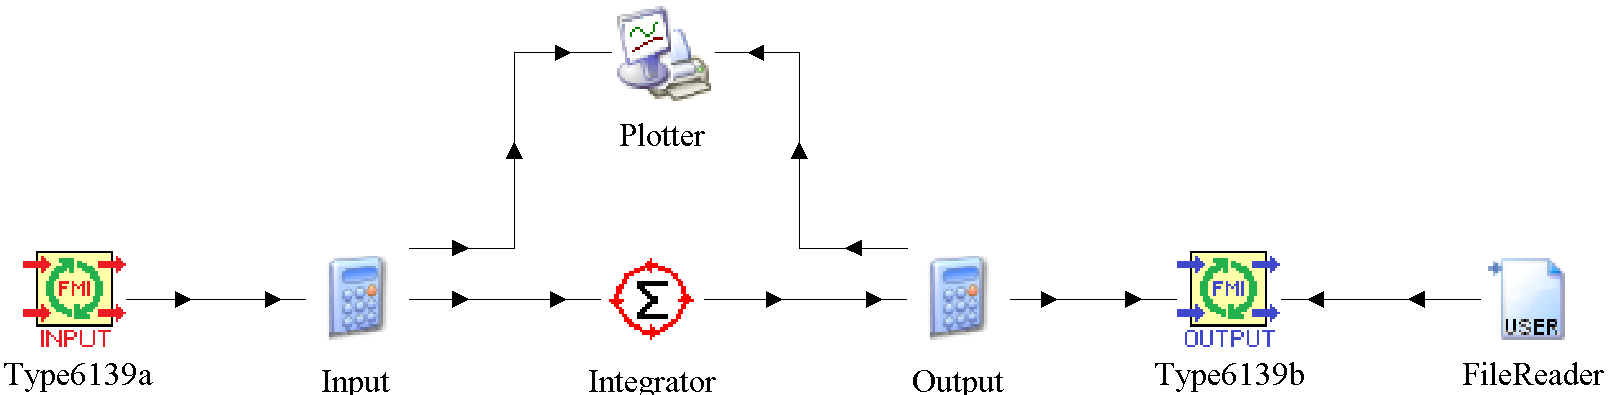
\includegraphics[width=0.95\textwidth]{trnsys_model}}
\caption{Example \trnsys model}
\label{fig:trnsys_model}
\end{figure}

\subsection{Configuring \typea}
With the help of Simulation Studio, configuration of \typea is simple:
\begin{itemize}
  \item Add the type to the model (via drag and drop from the toolbar on the right).
  \item Double-click the type icon to access its \emph{proforma}.
  There are 3 important tabs:
  \begin{itemize}
    \item \emph{Parameter tab}: Enter the number of FMU inputs, i.e., the number of inputs from the master algorithm to the \trnsys model.
    \item \emph{Output tab}: According to the number of FMU inputs defined in the Parameter tab, a list of type outputs is displayed here.
    These type outputs can be arbitrarily renamed.
    \item \emph{Special cards tab}: Provide the names of the FMU inputs as comma separated list in row~3.
    Alternatively, a file name can be provided (see below). 
    These names will be used for declaring the FMU inputs in the XML model description.
    These names can be different from the names defined in the Output tab, but the number of type output names and FMU input names must match.
    The first name in this list corresponds to the first type output, the second name in this list corresponds to the second type output and so forth. 
    \emph{Attention}: Do not change the values in row~1 and~2.
  \end{itemize}
\end{itemize}

When providing a file name for defining the FMU input names, the associated file is expected to have one entry per line, each corresponding to one FMU input name.
Like in the case of a comma separated list, the first entry corresponds to the first type output, the second entry corresponds to the second type output and so forth.
The file may contain comments and comment lines, which are indicated with a leading semicolon~(;).
\emph{Attention}: When using a file for defining FMU input names, this file has to be specified as additional file when exporting the FMU (see Section~\ref{sec:export:command}).

The output variables of \typea can be connected to other \trnsys types in the usual way.

\subsection{Configuring \typeb}
With the help of Simulation Studio, configuration of \typeb is simple:
\begin{itemize}
  \item Add the type to the model (via drag and drop from the toolbar on the right).
  \item Double-click the type icon to access its \emph{proforma}. There are 3 important tabs:
  \begin{itemize}
    \item \emph{Parameter tab}: Enter the number of FMU outputs, i.e., the number of outputs from \trnsys model to the the master algorithm .
    \item \emph{Input tab}: According to the number of FMU outputs defined in the Parameter tab, a list of type inputs is displayed here.
    These type inputs can be arbitrarily renamed.
    \item \emph{Special cards tab}: Provide the names of FMU outputs as comma separated list in row~3.
    Alternatively, a file name can be provided (see below).
    These names will be used for declaring the FMU outputs in the XML model description.
    These names can be different from the names defined in the Input tab, but the number of type input names and FMU output names must match.
    The first name in this list corresponds to the first type input, the second name in this list corresponds to the second type input and so forth.
    \emph{Attention}: Do not change the values in row~1 and~2.
  \end{itemize}
\end{itemize} 

When providing a file name for defining the FMU output names, the associated file is expected to have one entry per line, each corresponding to one FMU output name.
Like in the case of a comma separated list, the first entry corresponds to the first type input, the second entry corresponds to the second type input and so forth.
The file may contain comments and comment lines, which are indicated with a leading semicolon~(;).
\emph{Attention}: When using a file for defining FMU output names, this file has to be specified as additional file when exporting the FMU (see Section~\ref{sec:export:command}).

The input variables of \typeb can be connected to other \trnsys types in the usual way.

\clearpage

\section{Exporting an FMU using the graphical user interface}
\label{sec:export:gui}

Once a \trnsys model according to Section~\ref{sec:export:model} has been created, an FMU can be created with the following steps:
\begin{enumerate}
  \item \textbf{Specify the simulation time and step size.} Either click the \textit{Control cards} icon in the side bar on the left or select from the menu bar on the top \textit{Assembly}~$\rightarrow$~\textit{Control cards}. 
  Specify the values for \textit{Simulation start time}, \textit{Simulation stop time} and \textit{Simulation time step}.
  Regardless of the time units chosen here, the final FMU will always interpret time in seconds.
  \item \textbf{Create the deck file.} Either click the \textit{Write input file} icon in the side bar on the left or select from the menu bar on the top \textit{Calculate}~$\rightarrow$~\textit{Create input file}.
  \item \textbf{Run}~\textbf{\texttt{trnsys\_fmu\_create.exe}}.
  The FMU can be generated with the graphical user interface, see Figure~\ref{fig:trnsys_fmu_create_gui}
  To run it, simply double-click \texttt{trnsys\_fmu\_create.exe} in the installation directory and provide the necessary inputs:\\
  \textit{Mandatory input arguments}:
  \begin{itemize}
    \item \textbf{FMI model identifier}: Specify the FMU model identifier. 
    \emph{Attention}: The FMU model identifier must fulfill the restrictions for C function names!
    \item \textbf{TRNSYS deck file} Path to \trnsys deck file (absolute or relative).
  \end{itemize}
  \textit{Optional input arguments}:
  \begin{itemize}
    \item \textbf{Additional arguments}:
    \begin{itemize}
      \item Additional files may be specified (e.g., weather data or input/output name lists) that will be automatically copied to the FMU. The specified files paths may be absolute or relative.
      \item Start values for variables may be defined. For instance, to set variable with name \verb!var1! to value 12.34, specify \verb!var1=12.34! as optional argument.
    \end{itemize}
    \item \textbf{FMI version}: Specify FMI version (default: 2).
    \item \textbf{TRNSYS installation directory}: Absolute path to \trnsys installation directory. This should normally be set during the installation process (see Section~\ref{sec:install}).
    \item \textbf{Verbosity}: Turn on log messages.
    \item \textbf{Litter}: Do not clean-up intermediate files (e.g., log file with debug messages from Visual Studio compiler).
  \end{itemize}
\end{enumerate}

\begin{figure}[h]
\centering{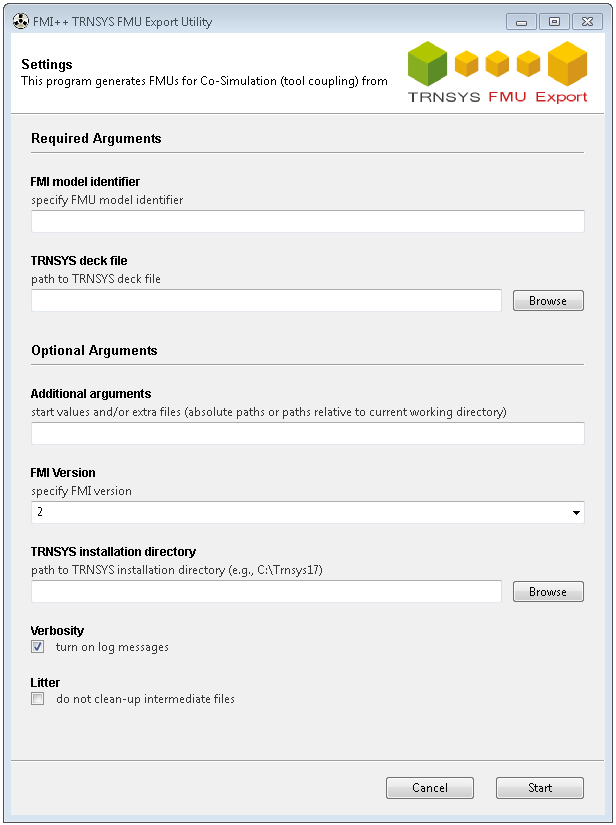
\includegraphics[width=0.98\textwidth]{trnsys_fmu_create_gui}}
\caption{The graphical user interface for creating an FMU.}
\label{fig:trnsys_fmu_create_gui}
\end{figure}

\clearpage

\section{Exporting an FMU using Python scripts}
\label{sec:export:command}

Instead of using the graphical user interface described in Chapter~\ref{sec:export:gui}, FMUs can also be generated using the \python script~\texttt{trnsys\_fmu\_create.py}, located in the installation directory.
The FMU is created by executing the script from the command prompt window (please refer to the \href{https://docs.python.org/2/faq/windows.html}{\python~FAQ} in case you need assistance with this).
Open the command prompt window, change to the directory containing the deck file and execute the script:
\begin{verbatim}
python <path_to_trnsys_fmu_dir>trnsys_fmu_create.py [-h] [-v] 
     -m <model_id> -d <deck_file> [-t <trnsys_install_dir>]
     [-f <fmi_version>] [<additional_file_1> ... <additional_file_N>]
     [var1=start_val1 ... varN=start_valN]
  \end{verbatim}
The path to the installation directory \verb!<path_to_trnsys_fmu_dir>! may be relative or absolute.
Optional arguments are enclosed by squared brackets \verb![!$\,$\ldots\verb!]!.

\textit{Mandatory input arguments}:
\begin{itemize}

  \item \verb!-m, --model-id!: Specify the FMU model identifier. \emph{Attention}: The FMU model identifier must fulfill the restrictions for C function names!
  \item \verb!-d, --deck-file!: Path to \trnsys deck file (absolute or relative).

\end{itemize}
\textit{Optional input arguments}:
\begin{itemize}

  \item \verb!-h, --help!: Display the help screen.
  \item \verb!-v, --verbose!: Turn on log messages.
  \item \verb!-l, --litter!: Do not clean-up intermediate files (e.g., log file with debug messages from Visual Studio compiler).
  \item \verb!-t, --trnsys-install-dir!: Absolute path to \trnsys installation directory. This should normally be set during the installation process (see Section~\ref{sec:install}).
  \item \verb!-f, --fmi-version!: Specify FMI version (\verb!1! or \verb!2!, default is \verb!2!)
  \item Additional files may be specified (e.g., weather data or input/output name lists) that will be automatically copied to the FMU. The specified files paths may be absolute or relative.
  \item Start values for variables may be defined. For instance, to set variable with name \verb!var1! to value 12.34, specify \verb!var1=12.34! in the command line as optional argument.

\end{itemize}